% Provenance (never printed): old terminale S material on the early Earth (the
% primitive atmosphere and its outgassing, the first traces of life, the rise of
% oxygen read in the rocks: banded iron formations, red beds) and the faint young
% Sun. Owner (Sync 0/1): outgassing and primitive atmosphere, faint young Sun
% problem, stromatolite, Great Oxidation Event, banded iron formation, red beds.
% Recalled: age of the Earth (g12.07), zircons (g12.01), equilibrium temperature
% (g10.02), photosynthesis and cyanobacteria (biology), air composition, greenhouse
% gases as molecules and redox (chemistry). Figures: figdata/grade-12/early_earth.py.
\chapter{الأرض الفتية وغلافها الجوي}\label{ch:g12:early-earth}

في سلاسل هامرسلي في شمال غرب أستراليا، تبدو جدران خانق دايلز
مخططة كقالب حلوى من طبقات: أشرطة رقيقة من صخر أحمر ورمادي وأسود. إنها
تكوين حديد شريطي، ترسّب على قاع بحر قبل أكثر من 2.5 مليار
سنة.
وقد صدئ الحديد الذي فيها في ذلك البحر، والصدأ يحتاج إلى الأكسجين. يسأل هذا
الفصل كيف كانت الأرض الفتية وهواؤها، وكيف تسجل الصخور
اللحظة التي ظهر فيها الأكسجين.
% ledger: dbca:karijini, earle:bif, photo:g12-dales-gorge

\begin{omfigure}
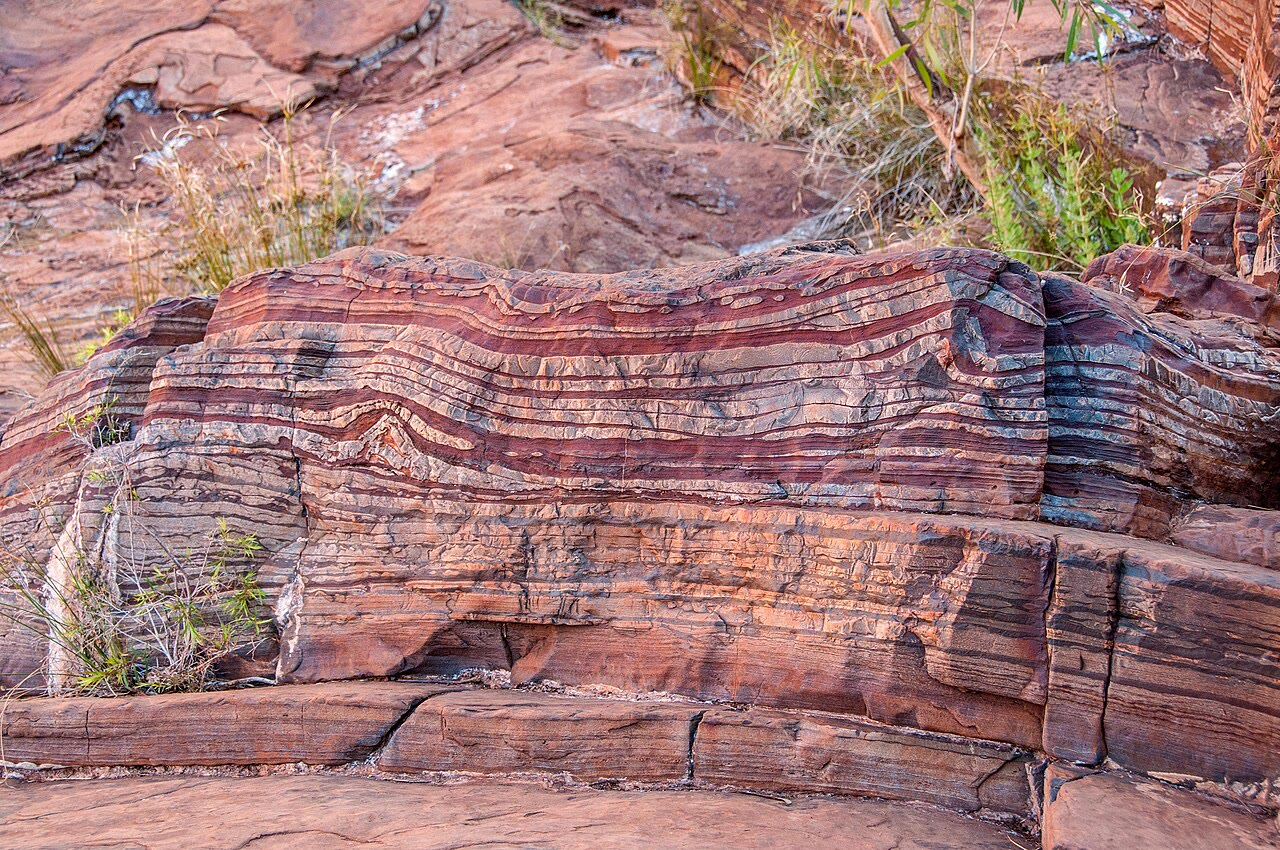
\includegraphics[width=0.72\linewidth]{images/book2/g12-dales-gorge-bif.jpg}

{\small تكوين حديد شريطي عند شلالات فورتسكيو، خانق دايلز، منتزه كاريجيني
الوطني، غرب أستراليا. الصورة: غرايم تشرتشارد، CC~BY~2.0
(ويكيميديا كومنز).}
\end{omfigure}

\begin{recall}
\omterm{def:g12:age-of-the-earth:age}{عمر الأرض} 4.54 مليار سنة (\cref{ch:g12:age-of-the-earth})،
وتُظهر حبيبات الزركون أن قشرة كانت موجودة قبل 4.4 مليار سنة
(\cref{ch:g12:continental-crust}). \omterm{def:g10:habitable-planet:equilibrium-temperature}{ودرجة حرارة التوازن} لكوكب ما،
$T_{\mathrm{eq}} = \left(S(1-A)/(4\sigma)\right)^{1/4}$، تبلغ نحو \qty{255}{K}
للأرض اليوم (\cref{ch:g10:habitable-planet}). والهواء الجاف اليوم
\qty{78}{\percent} منه نيتروجين و\qty{21}{\percent} أكسجين، وثاني أكسيد الكربون
والميثان غازات دفيئة؛ والعنصر الذي يأخذ الأكسجين يتأكسد (كتب
الكيمياء). والنباتات والطحالب والبكتيريا الزرقاء تصنع غذاءها بالتمثيل
الضوئي، الذي يطلق الأكسجين (كتب الأحياء).
\end{recall}
% ledger: usgs:age-earth (Book 1 row), wilde01:zircon, earth:TSI, earth:albedo, air:N2, air:O2

\section{الأرض الفتية}

نمت الأرض بتراكم أجسام أصغر. وبعد نحو 60 مليون سنة
من بدء تكوّن المجموعة الشمسية، اصطدم بها جسم ربما في حجم المريخ،
فكوّنت المادة المقذوفة في الفضاء القمر. وكانت الأرض الفتية
ساخنة ولا تزال منصهرة جزئيًا. ثم بردت، وبحلول نحو 4.4 مليار سنة مضت
كانت لها قشرة ومحيط: فحبيبات الزركون التي في ذلك العمر تحمل البصمة الكيميائية
للماء السائل.
% ledger: nasa:moon-formation, wilde01:zircon

\section{الغلاف الجوي البدائي}

\begin{definition}[انطلاق الغازات؛ الغلاف الجوي البدائي]\label{def:g12:early-earth:primitive-atmosphere}
\emph{انطلاق الغازات}\index{انطلاق الغازات} هو تحرر الغازات الذائبة في
الصهارة، عبر البراكين وعبر الأرض. و\emph{الغلاف الجوي
البدائي}\index{غلاف جوي بدائي} هو الغلاف الجوي للأرض قبل أن
تغيّره الكائنات الحية: وقد بُني أساسًا بانطلاق الغازات، فكان يحوي النيتروجين
وثاني أكسيد الكربون وبخار الماء، وثاني أكسيد كربون أكثر مما اليوم، ولا يكاد
يحوي أكسجينًا حرًا.
\end{definition}
% ledger: usgs:volcanic-gases (Book 1 row), holland06:stages (stage 1 anoxic), feulner12:fys (more carbon dioxide)

لا تزال البراكين تُظهر كيف يتكوّن غلاف جوي كهذا: فحين تصعد الصهارة وينخفض
الضغط، تفلت غازاتها الذائبة، وأوفرها على الإطلاق
بخار الماء، ثم ثاني أكسيد الكربون. والنيتروجين وثاني أكسيد الكربون، الغازان
اللذان سادا الهواء البدائي، لا يزالان أهم غازات البراكين الحاملة للنيتروجين
وللكربون اليوم. وقد تكاثف بخار الماء فصار
المحيط. أما الأكسجين فكان أقل من \qty{0.001}{\percent} من مستواه في هواء
اليوم.
% ledger: usgs:volcanic-gases (Book 1 row), pk02:anoxic

كانت الشمس الفتية أقل سطوعًا مما هي اليوم. فبينما تحوّل الهيدروجين إلى
هيليوم في لبّها، ينكمش اللب ويسخن، فتزداد قدرة الشمس
ببطء.

\begin{proposition}[لمعان الشمس الفتية]\label{prop:g12:early-earth:luminosity}
إذا كان $t_\odot$ عمر الشمس الحالي و$L_\odot$ لمعانها
الحالي، فإن لمعانها حين كان عمرها $t$ سنة كان
\[
  L(t) = \frac{L_\odot}{1 + \frac{2}{5}\left(1 - t/t_\odot\right)} .
\]
\end{proposition}
% ledger: gough81:luminosity, connelly12:cai

هذا التقريب لنماذج الشمس المحسوبة مسلَّم به هنا. فعند
ولادة الشمس، $t = 0$، يعطي $L = L_\odot/1.4 \approx 0.71\,L_\odot$:
فقد كانت الشمس الفتية أخفت بنحو \qty{30}{\percent}.

\begin{example}[الأرض قبل أربعة مليارات سنة]\label{ex:g12:early-earth:young-sun}
خذ $t_\odot = 4.567$ مليار سنة. قبل أربعة مليارات سنة كان عمر الشمس
0.567 مليار سنة، إذن $1 - t/t_\odot = 4/4.567 \approx 0.876$
و$L \approx L_\odot/1.350 \approx 0.741\,L_\odot$. وكان ضوء الشمس الذي يبلغ
الأرض $0.741 \times 1361 \approx \qty{1008}{W/m^2}$. ومع الإبقاء على \omterm{def:g10:earth-energy-budget:albedo}{ألبيدو}
اليوم، تتناسب \omterm{def:g10:habitable-planet:equilibrium-temperature}{درجة حرارة التوازن} مع الجذر الرابع لضوء
الشمس: $255 \times 0.741^{1/4} \approx 255 \times 0.928 \approx
\qty{237}{K}$، أي نحو \qty{-36}{\celsius}.
\end{example}
% values: L_4Ga 0.7406, S_4Ga 1007.9, Teq_today 255.1, Teq_4Ga 236.7 (early_earth.py)

\begin{omfigure}
\begin{tikzpicture}
\begin{axis}[omrecord, scale only axis, width=0.66\linewidth, height=4.6cm,
  xmin=0, xmax=4.6, ymin=225, ymax=295, x dir=reverse, axis y line*=left,
  xlabel={\foreignlanguage{arabic}{الزمن قبل الحاضر بمليارات السنين}}, ylabel={\foreignlanguage{arabic}{درجة الحرارة \babelsublr{(K)}}},
  xtick={0,0.5,...,4.5}, x tick label style={/pgf/number format/.cd, fixed, precision=1}]
% computed in figdata/grade-12/early_earth.py; ledger: gough81:luminosity, earth:TSI, earth:albedo, earth:Tsurf
\addplot[omDef, line width=1.2pt] table[x=t_Ga, y=Teq] {figdata/out/grade-12-early_earth-sun.dat};
\addplot[omThm, densely dashed, domain=0:4.6, samples=2] {273.15};
\addplot[black!60, densely dotted, domain=0:4.6, samples=2] {288};
\coordinate (teq) at (axis cs:2.6,239);
\coordinate (frz) at (axis cs:2.3,274);
\coordinate (sfc) at (axis cs:2.3,289);
\end{axis}
\begin{axis}[omrecord, scale only axis, width=0.66\linewidth, height=4.6cm,
  xmin=0, xmax=4.6, ymin=0.65, ymax=1.05, x dir=reverse, axis y line*=right, axis x line=none,
  ylabel={\foreignlanguage{arabic}{لمعان الشمس بوحدة $L_\odot$}}, ymajorgrids=false, xmajorgrids=false,
  y tick label style={/pgf/number format/.cd, fixed, fixed zerofill, precision=2}]
\addplot[omProp, line width=0.9pt, densely dashdotted] table[x=t_Ga, y=L] {figdata/out/grade-12-early_earth-sun.dat};
\coordinate (lum) at (axis cs:1.7,0.86);
\end{axis}
\node[font=\scriptsize, text=omDef, anchor=north] at (teq) {درجة حرارة التوازن};
\node[font=\scriptsize, text=omThm, anchor=south] at (frz) {\foreignlanguage{arabic}{يتجمد الماء، \babelsublr{\qty{273}{K}}}};
\node[font=\scriptsize, text=black!70, anchor=south] at (sfc) {\foreignlanguage{arabic}{متوسط السطح اليوم، \babelsublr{\qty{288}{K}}}};
\node[font=\scriptsize, text=omProp, anchor=north west] at (lum) {\foreignlanguage{arabic}{اللمعان، على المقياس الأيمن}};
\end{tikzpicture}

{\small الشمس الفتية الخافتة: لمعانها (المقياس الأيمن) \omterm{def:g10:habitable-planet:equilibrium-temperature}{ودرجة حرارة التوازن}
للأرض مع \omterm{def:g10:earth-energy-budget:albedo}{ألبيدو} اليوم (المقياس الأيسر)، رجوعًا إلى ولادة
الشمس. حُسبت من غوف (1981) مع ضوء الشمس \omterm{def:g10:earth-energy-budget:albedo}{والألبيدو} الحاليين.}
\end{omfigure}

\begin{definition}[مشكلة الشمس الفتية الخافتة]\label{def:g12:early-earth:faint-young-sun}
\emph{مشكلة الشمس الفتية الخافتة}\index{مشكلة الشمس الفتية الخافتة} هي
التناقض بين الشمس الأخفت في المليارات الأولى من \omterm{def:g12:age-of-the-earth:age}{عمر الأرض}،
التي كانت الأرض بغلافها الجوي الحالي ستتجمد تحتها، وبين
الصخور، التي تُظهر أن الماء السائل كان موجودًا.
\end{definition}
% ledger: feulner12:fys

شاعت هذه المشكلة في عام 1972 على يد كارل ساغان وجورج مولن،
اللذين اقترحا أثر دفيئة أقوى جوابًا لها. ومعظم الأجوبة
المدروسة منذ ذلك الحين تلجأ إلى مزيد من غازات الدفيئة في \omterm{def:g12:early-earth:primitive-atmosphere}{الغلاف الجوي البدائي}:
ثاني أكسيد كربون أكثر بكثير مما اليوم، أو ميثان صنعته الميكروبات الأولى، أو
كليهما. ففي حساب كلاسيكي، يكفي نحو عُشر بار من ثاني أكسيد الكربون،
مع قليل من الميثان، لإبقاء الأرض الفتية دافئة كما هي اليوم؛ ودون
الميثان، يلزم نحو ثلاثة أضعاف ذلك. ولا تُعد المشكلة بعدُ
محلولة.
% ledger: feulner12:fys

\section{الحياة والأكسجين}

يغطي السجل الأحفوري \omterm{def:g12:early-earth:stromatolite}{للستروماتوليتات} قرابة \num{3500} مليون سنة:
فهي من أقدم علامات الحياة.

\begin{definition}[الستروماتوليت]\label{def:g12:early-earth:stromatolite}
\emph{الستروماتوليت}\index{ستروماتوليت} كومة طبقية يبنيها في
المياه الضحلة بساط من الميكروبات، أساسًا البكتيريا الزرقاء، التي تحتجز
حبيبات الرسوبيات وتربطها وتجعل الكربونات تنمو، طبقة فوق طبقة.
\end{definition}
% ledger: noffke13:stromatolites

توجد \omterm{def:g12:early-earth:stromatolite}{ستروماتوليتات} أحفورية عمرها \num{3430} مليون سنة في صوان ستريلي
بول في بيلبارا، غرب أستراليا. وتنمو \omterm{def:g12:early-earth:stromatolite}{ستروماتوليتات} حية اليوم في
الماء الشديد الملوحة لبركة هاملين في خليج القرش، وهو أملح بمرتين من
ماء البحر المعتاد، حيث تُعد أشهر مثال حديث.
% ledger: allwood06:spc, noffke13:stromatolites, dbca:hamelin

\begin{omfigure}
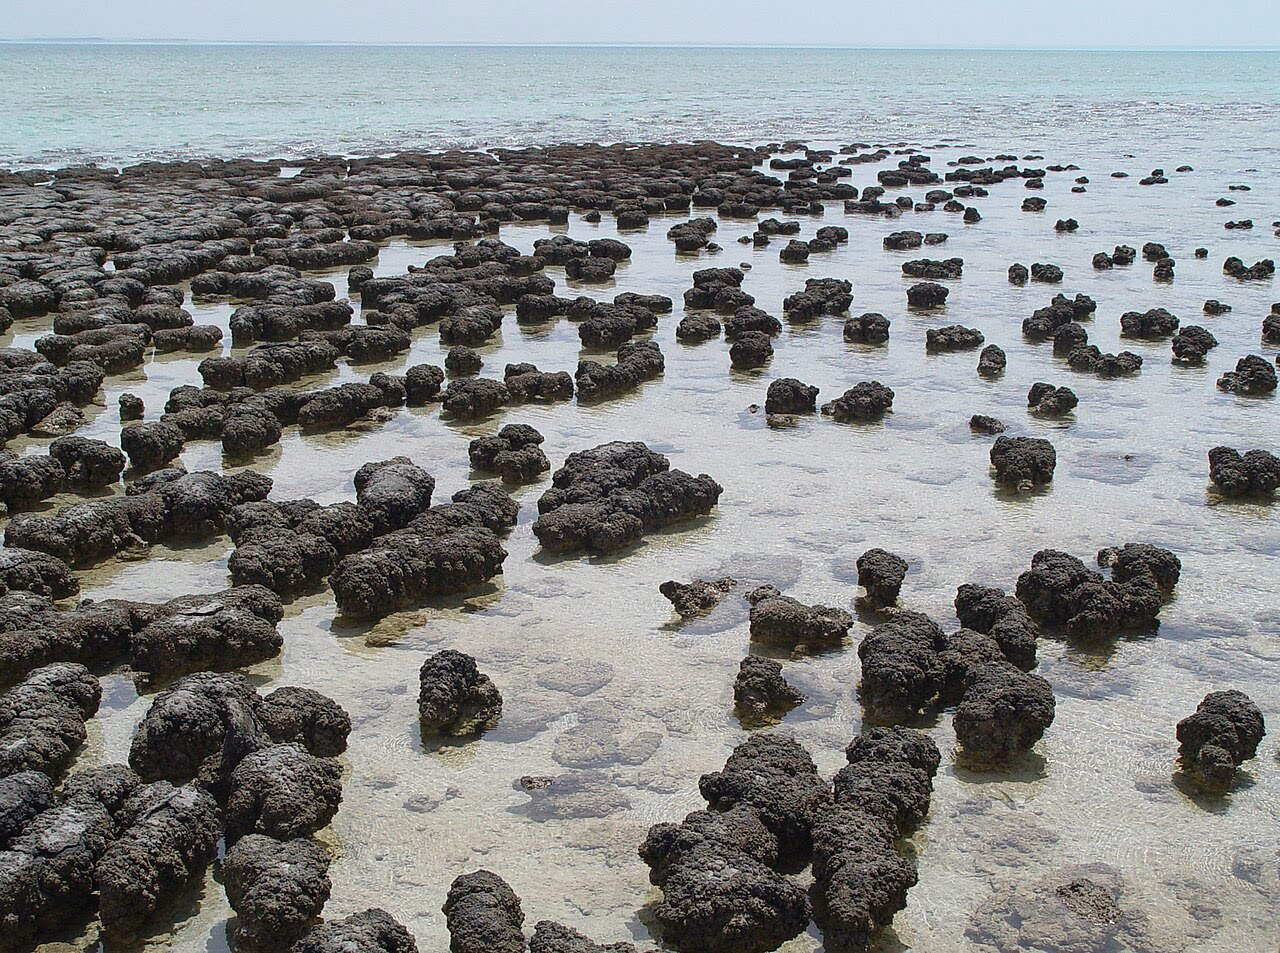
\includegraphics[width=0.6\linewidth]{images/book2/g12-shark-bay-stromatolites.jpg}

{\small \omterm{def:g12:early-earth:stromatolite}{ستروماتوليتات} حية في بركة هاملين، خليج القرش، غرب أستراليا.
الصورة: بول هاريسون، CC~BY-SA~3.0 (ويكيميديا كومنز).}
\end{omfigure}
% ledger: photo:g12-shark-bay

جاءت البكتيريا الزرقاء بشيء جديد: تمثيل ضوئي يطلق
الأكسجين. لكن الأكسجين الذي صنعته لم يبقَ في الهواء زمنًا طويلًا. فقد
كان يُستهلك بالسرعة التي يُصنع بها: بالحديد الذائب في البحر،
وبالكبريت وبالميثان.

\section{صعود الأكسجين}

قبل الأكسجين، كان الحديد يستطيع أن ينتقل ذائبًا في ماء البحر على هيئة الأيون
\ce{Fe^2+}. فيحوّله الأكسجين إلى الحديد(III)، الذي لا يذوب: فيسقط
إلى القاع رسوبًا صدئًا.

\begin{proposition}[الحديد يأخذ الأكسجين]\label{prop:g12:early-earth:iron}
يتأكسد الحديد(II) الذائب بالأكسجين في الماء إلى هيدروكسيد الحديد(III)،
الذي يترسب:
\[
  \ce{4Fe^2+ + O2 + 10H2O -> 4Fe(OH)3 + 8H+} .
\]
كل جزيء من الأكسجين يزيل أربعة أيونات من الحديد الذائب؛ وما دام
الحديد الذائب باقيًا، يُستهلك الأكسجين المصنوع.
\end{proposition}
% ledger: earle:bif (ferrous iron oxidised to insoluble ferric iron)

\begin{proof}
تحقق من الموازنة. الحديد: 4 في كل طرف. الأكسجين: $2 + 10 = 12$ في اليسار،
و$4 \times 3 = 12$ في اليمين. الهيدروجين: $20$ في اليسار، و$4 \times 3 + 8 =
20$ في اليمين. الشحنة: $4 \times (+2) = +8$ في اليسار، و$8 \times (+1) =
+8$ في اليمين.
\end{proof}

\begin{definition}[تكوين الحديد الشريطي]\label{def:g12:early-earth:bif}
\emph{تكوين الحديد الشريطي}\index{تكوين الحديد الشريطي} صخر
رسوبي من طبقات رقيقة متناوبة من أكاسيد الحديد، مثل
الهيماتيت، ومن الصوان، وهو سيليكا دقيقة الحبيبات فقيرة بالحديد. وكلها تقريبًا
أقدم من 1.8 مليار سنة.
\end{definition}
% ledger: earle:bif, holland06:stages

تحتاج \omterm{def:g12:early-earth:bif}{تكوينات الحديد الشريطية} إلى ماءين معًا: \omterm{def:g10:layered-ocean:thermocline}{محيط عميق} خالٍ من الأكسجين،
يحمل الحديد الذائب، وبحر ضحل مشمس تصنع فيه البكتيريا الزرقاء
الأكسجين فيترسب الحديد. وهي شائعة في الصخور التي عمرها من 2.4 إلى
1.8 مليار سنة، وتكوينات سلاسل هامرسلي أقدم من ذلك أيضًا.
\omterm{def:g12:early-earth:bif}{وتكوينات الحديد الشريطية} خام شائع للحديد.
% ledger: earle:bif, holland06:stages (Archean BIF, Hamersley), dbca:karijini

\begin{omfigure}
\begin{tikzpicture}[x=1cm, y=1cm, font=\scriptsize]
  % sea and floor
  \fill[omSea] (0,0) rectangle (11,4);
  \fill[omSea!45!white] (0,2.9) rectangle (11,4);
  \draw[omDef!60, line width=0.4pt, densely dashed] (0,2.9) -- (11,2.9);
  \node[anchor=north east, text=omDef] at (10.9,3.95) {مياه سطحية مشمسة};
  \node[anchor=south east, text=omDef, align=right] at (10.9,0.12) {مياه عميقة\\خالية من الأكسجين\\\foreignlanguage{arabic}{غنية بأيونات \ce{Fe^2+}}};
  % floor with layers
  \foreach \i/\c in {0/red!55!black, 1/black!20, 2/red!55!black, 3/black!20, 4/red!55!black, 5/black!20} {
    \fill[\c] (0,-0.12*\i) rectangle (11,-0.12*\i-0.12);
  }
  \draw[black!60] (0,0) -- (11,0);
  \node[anchor=west] at (11.1,0.02) {أكسيد الحديد};
  \node[anchor=west] at (11.1,-0.44) {الصوان};
  \draw[black!50, line width=0.3pt] (11.05,0.02) -- (10.6,-0.06);
  \draw[black!50, line width=0.3pt] (11.05,-0.44) -- (10.6,-0.30);
  % upwelling iron
  \foreach \x in {0.5,1.0,1.5} {
    \draw[-{Stealth}, omDef, line width=0.8pt] (\x,0.4) .. controls (\x+0.4,1.5) and (\x+0.6,2.2) .. (\x+0.9,2.85);
  }
  \node[text=omDef, anchor=west] at (2.3,1.3) {\foreignlanguage{arabic}{يصعد \ce{Fe^2+}}};
  % cyanobacteria and oxygen
  \foreach \x in {3.8,4.4,5.0,5.6,6.2} {\fill[green!45!black] (\x,3.35) circle (0.07);}
  \node[anchor=south, text=green!35!black] at (5.0,3.47) {\foreignlanguage{arabic}{البكتيريا الزرقاء تصنع \ce{O2}}};
  % reaction
  \node[draw=black!40, fill=white, rounded corners=2pt, inner sep=2pt] at (5.4,2.45) {\ce{4Fe^2+ + O2 + 10H2O -> 4Fe(OH)3 + 8H+}};
  % falling rust
  \foreach \x/\y in {4.6/1.9, 5.0/1.5, 5.5/1.8, 5.9/1.2, 4.3/1.1, 5.2/0.7, 6.1/0.6} {\fill[red!60!black] (\x,\y) circle (0.06);}
  \draw[-{Stealth}, red!60!black, line width=0.6pt] (6.6,2.1) -- (6.6,0.25);
  \node[anchor=west, text=red!60!black, align=left] at (6.7,1.75) {الحديد الثلاثي يترسب\\طبقةً صدئة};
\end{tikzpicture}

{\small كيف يتكوّن \omterm{def:g12:early-earth:bif}{تكوين الحديد الشريطي} (رسم تخطيطي، ليس بمقياس رسم): الحديد
الذائب في المياه العميقة، الخالية من الأكسجين، يصعد إلى البحر
المشمس، حيث يحوّله الأكسجين الذي تصنعه البكتيريا الزرقاء إلى الحديد(III)، الذي
يترسب. فتتناوب طبقات غنية بالحديد مع طبقات من الصوان.}
\end{omfigure}

ثم بدأ الأكسجين يبقى في الهواء.

\begin{definition}[حدث الأكسدة العظيم]\label{def:g12:early-earth:goe}
\emph{حدث الأكسدة العظيم}\index{حدث الأكسدة العظيم} هو
الفترة الممتدة من نحو \num{2.46} إلى نحو \num{2.06} مليار سنة مضت، التي
تراكم فيها الأكسجين الحر لأول مرة في الغلاف الجوي للأرض وفي البحار الضحلة،
فبلغ ربما عُشر مستواه الحالي.
\end{definition}
% ledger: gumsley17:goe, holland06:stages (0.02-0.04 atm, about a tenth of 0.21)

الدليل في الصخور. فبعض المعادن، ومنها البيريت
واليورانينيت، يدمرها الأكسجين؛ ومع ذلك توجد حبيبات منها دحرجتها الأنهار
في رسوبيات قديمة، وتغيب حبيبات البيريت عن الرسوبيات التي ترسبت
بعد صعود الأكسجين. ونظائر الكبريت في الصخور الأقدم من نحو 2.45 مليار سنة تحمل
بصمة لا يتركها إلا هواء فيه أقل من جزء من مئة ألف من أكسجين
اليوم؛ وبحلول 2.09 مليار سنة مضت تكون قد اختفت. وعلى اليابسة ظهرت
\omterm{def:g12:early-earth:red-beds}{الطبقات الحمراء}.
% ledger: kasting25:indicators, pk02:anoxic, farquhar00:sulfur

\begin{definition}[الطبقات الحمراء]\label{def:g12:early-earth:red-beds}
\emph{الطبقات الحمراء}\index{طبقات حمراء} صخور رسوبية --- أحجار رملية
وأحجار غرينية وسجيل --- يلوّنها بالأحمر غشاء من أكسيد الحديد(III)،
الهيماتيت، على حبيباتها. ولا تتكوّن إلا حيث يكفي الأكسجين
لأكسدة الحديد.
\end{definition}
% ledger: kasting25:indicators (redbeds an oxygen indicator)

\begin{omfigure}
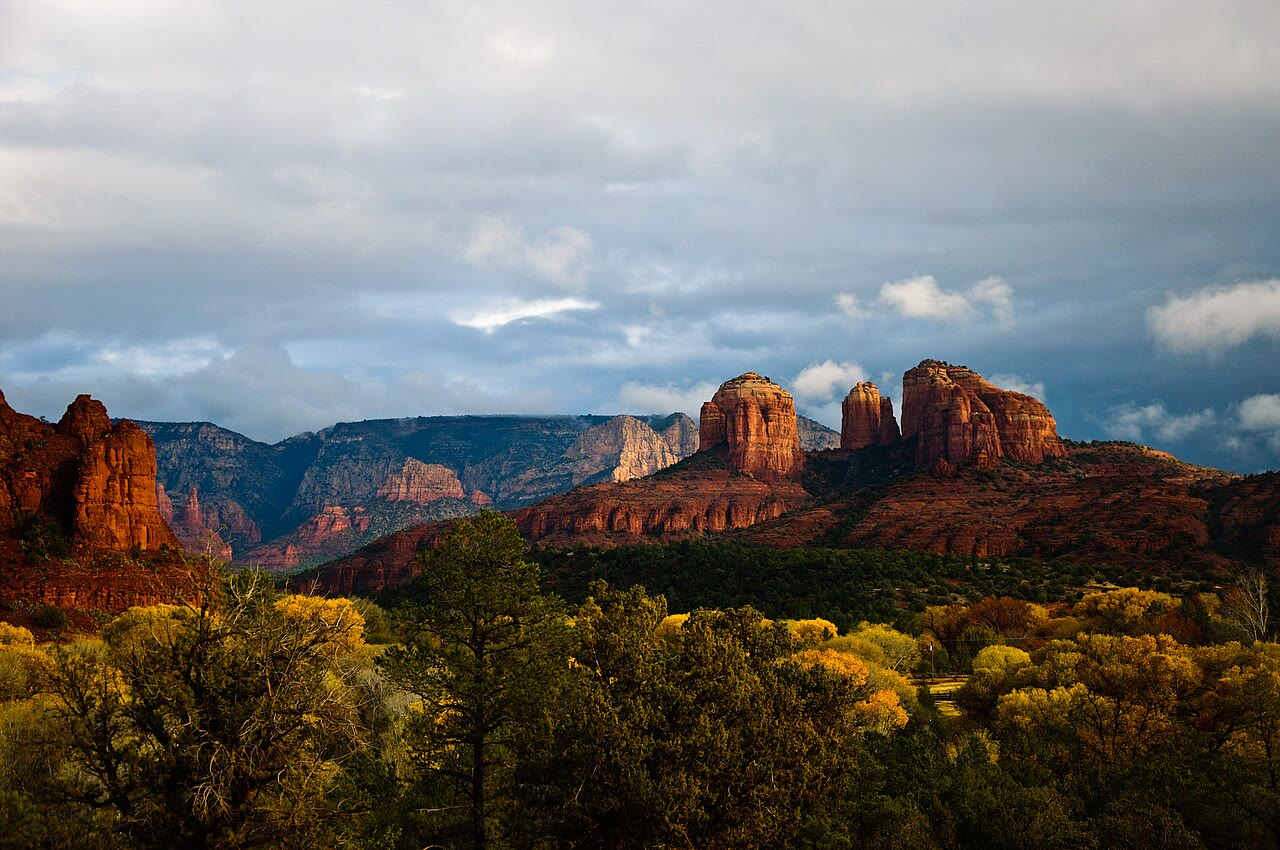
\includegraphics[width=0.66\linewidth]{images/book2/g12-sedona-red-beds.jpg}

{\small \omterm{def:g12:early-earth:red-beds}{طبقات حمراء}: صخرة الكاتدرائية قرب سيدونا، أريزونا، المبنية من أحجار رملية
حمراء من العصر البرمي. الصورة: ويندي من بنسلفانيا، CC~BY-SA~2.0 (ويكيميديا
كومنز).}
\end{omfigure}
% ledger: photo:g12-sedona, azgs:cathedral (Permian Schnebly Hill Sandstone)

توقف تكوّن \omterm{def:g12:early-earth:bif}{تكوينات الحديد الشريطية} في جوهره بعد 1.8 مليار
سنة مضت: فقد صار في \omterm{def:g10:layered-ocean:thermocline}{المحيط العميق} أيضًا حينئذ من الأكسجين ما يكفي ليكفّ عن حمل
الحديد. وعلى مدى المليار سنة التالية تغيّر الأكسجين قليلًا؛ وبعد 0.85 مليار
سنة مضت تراكم من جديد، نحو \qty{21}{\percent} اليوم.
% ledger: earle:bif, holland06:stages

\begin{method}[قراءة خط زمني جيولوجي]\label{met:g12:early-earth:timeline}
\begin{enumerate}
  \item جد الاتجاه الذي يجري فيه الزمن على المحور، ووحدته (ملايين أو
        مليارات السنين قبل الحاضر).
  \item حدد الدهور على الشريط الملوّن، واقرأ حدودها.
  \item لكل حدث، اقرأ تاريخه، أو الفترة التي
        وقع فيها، وقل أي سجل يؤرّخه (معدن، أو أحفورة، أو صخر).
  \item احسب المُدد بالطرح، وقارنها \omterm{def:g12:age-of-the-earth:age}{بعمر
        الأرض}.
  \item تحقق من الترتيب: فالنتيجة يجب ألا تسبق سببها.
\end{enumerate}
\end{method}

\begin{omfigure}
\begin{tikzpicture}
\begin{axis}[omrecord, width=0.82\linewidth, height=6.2cm, ymode=log, xmin=0, xmax=4.6, ymin=1e-7, ymax=5,
  x dir=reverse, xlabel={\foreignlanguage{arabic}{الزمن قبل الحاضر بمليارات السنين}}, ylabel={\foreignlanguage{arabic}{الأكسجين في الهواء، وقيمة اليوم $=1$}},
  xtick={0,0.5,...,4.5}, x tick label style={/pgf/number format/.cd, fixed, precision=1},
  ytick={1e-6,1e-4,1e-2,1}, ymajorgrids=true, xmajorgrids=false, clip=false]
% computed in figdata/grade-12/early_earth.py (schematic through the sourced bounds); ledger: holland06:stages, pk02:anoxic, gumsley17:goe, ics:base.Hadean, ics:base.Archean, ics:base.Proterozoic, ics:base.Paleozoic
\fill[omThm!12] (axis cs:2.46,1e-7) rectangle (axis cs:2.06,5);
\addplot[black, line width=1.2pt] table[x=t_Ga, y=pal] {figdata/out/grade-12-early_earth-oxygen.dat};
% eon band (ICS colours), below the axis
\fill[icsHadean] (axis cs:4.567,1.5e-7) rectangle (axis cs:4.031,4e-7);
\fill[icsArchean] (axis cs:4.031,1.5e-7) rectangle (axis cs:2.5,4e-7);
\fill[icsProterozoic] (axis cs:2.5,1.5e-7) rectangle (axis cs:0.5388,4e-7);
\fill[icsPhanerozoic] (axis cs:0.5388,1.5e-7) rectangle (axis cs:0,4e-7);
\node[font=\tiny, text=white] at (axis cs:4.30,2.45e-7) {الدهر الجهنمي};
\node[font=\tiny, text=white] at (axis cs:3.27,2.45e-7) {الدهر السحيق};
\node[font=\tiny, text=white] at (axis cs:1.52,2.45e-7) {دهر الحياة الطليعية};
% events
\draw[omDef, line width=0.6pt] (axis cs:4.4,4e-7) -- (axis cs:4.4,3e-3);
\node[font=\scriptsize, text=omDef, anchor=south west] at (axis cs:4.4,3e-3) {زركون وماء};
\draw[omMeth, line width=0.6pt] (axis cs:3.43,4e-7) -- (axis cs:3.43,1.2e-6);
\node[font=\scriptsize, text=omMeth, anchor=south] at (axis cs:3.43,1.2e-6) {أولى الستروماتوليتات};
\draw[red!60!black, line width=3pt] (axis cs:2.4,3e-6) -- (axis cs:1.8,3e-6);
\node[font=\scriptsize, text=red!60!black, anchor=north] at (axis cs:2.16,2.4e-6) {تكوينات الحديد الشريطية};
\node[font=\scriptsize, text=omThm, anchor=south, align=center] at (axis cs:2.26,1.2) {حدث الأكسدة\\العظيم};
\node[font=\scriptsize, anchor=south] at (axis cs:3.2,1.3e-5) {\foreignlanguage{arabic}{أقل من $10^{-5}$ من مستوى اليوم}};
\node[font=\scriptsize, anchor=south] at (axis cs:1.4,0.12) {نحو العُشر};
\end{axis}
\end{tikzpicture}

{\small الأكسجين في الهواء عبر الزمن (رسم تخطيطي، مقياس لوغاريتمي): يصل
المنحنى بين الحدود المقيسة ويخفي تقلبات السجل
الحقيقي. والفترة المظللة هي \omterm{def:g12:early-earth:goe}{حدث الأكسدة العظيم}؛ والشريط الأحمر يحدد
الزمن الذي كانت فيه \omterm{def:g12:early-earth:bif}{تكوينات الحديد الشريطية} شائعة، من 2.4 إلى 1.8 مليار سنة
مضت. والدهور من الجدول الكرونوستراتيغرافي
الدولي.}
\end{omfigure}

\section{تمارين}

\begin{exercise}[$\star$]\label{exo:g12:early-earth:1}
أعطِ المصطلح: (أ) تحرر الغازات الذائبة في الصهارة؛ (ب) كومة طبقية
يبنيها بساط ميكروبي؛ (ج) صخر من طبقات متناوبة من أكسيد الحديد
والصوان؛ (د) صخور رسوبية يلوّنها الهيماتيت؛ (ه) الفترة
التي تراكم فيها الأكسجين في الهواء لأول مرة.
\end{exercise}

\begin{exercise}[$\star$]\label{exo:g12:early-earth:2}
رتّب، من الأقدم: نهاية معظم \omterm{def:g12:early-earth:bif}{تكوينات الحديد الشريطية}؛ وأولى
\omterm{def:g12:early-earth:stromatolite}{ستروماتوليتات} بيلبارا؛ وحبيبات الزركون التي تُظهر الماء السائل؛ \omterm{def:g12:early-earth:bif}{وتكوينات
الحديد الشريطية} في هامرسلي؛ ونهاية \omterm{def:g12:early-earth:goe}{حدث الأكسدة العظيم}.
\end{exercise}

\begin{exercise}[$\star$]\label{exo:g12:early-earth:3}
باستعمال قانون اللمعان، احسب لمعان الشمس عند ولادتها، كسرًا
من لمعانها اليوم. بأي نسبة مئوية كانت أخفت؟
\end{exercise}

\begin{exercise}[$\star$]\label{exo:g12:early-earth:4}
توجد حبيبات بيريت دحرجتها الأنهار في رسوبيات قديمة، لكنها لا توجد في
الرسوبيات التي ترسبت بعد صعود الأكسجين. ماذا يخبرك ذلك عن
الهواء في زمن الرسوبيات القديمة؟ ولماذا؟
\end{exercise}

\begin{exercise}[$\star$]\label{exo:g12:early-earth:5}
سمِّ الغازين الأوفر بين الغازات التي تطلقها البراكين، وقل ما آل إليه
كل منهما في الأرض الفتية.
\end{exercise}

\begin{exercise}[$\star\star$]\label{exo:g12:early-earth:6}
احسب لمعان الشمس \omterm{def:g10:habitable-planet:equilibrium-temperature}{ودرجة حرارة التوازن} للأرض (اليوم
\qty{255}{K}، \omterm{def:g10:earth-energy-budget:albedo}{والألبيدو} دون تغيير) قبل 3 مليارات سنة وقبل 2.45 مليار
سنة، آخذًا $t_\odot = 4.567$ مليار سنة.
\end{exercise}

\begin{exercise}[$\star\star$]\label{exo:g12:early-earth:7}
كم يلزم من الأكسجين لترسيب \qty{1}{kg} من الحديد الذائب على هيئة
هيدروكسيد الحديد(III)؟ (الكتل المولية: الحديد \qty{55.85}{g/mol}، والأكسجين
\qty{16.00}{g/mol}.)
\end{exercise}

\begin{exercise}[$\star\star$]\label{exo:g12:early-earth:8}
مستعينًا بالخط الزمني، (1) كم دام \omterm{def:g12:early-earth:goe}{حدث الأكسدة العظيم}؟ (2)
في أي كسر من تاريخ الأرض لم يكن في الهواء أكسجين يُذكر؟
(3) كم من الزمن بعد أولى \omterm{def:g12:early-earth:stromatolite}{الستروماتوليتات} بدأ الأكسجين يتراكم؟
\end{exercise}

\begin{exercise}[$\star\star$]\label{exo:g12:early-earth:9}
يحوي كل من \omterm{def:g12:early-earth:bif}{تكوين الحديد الشريطي} والطبقة الحمراء أكسيد الحديد(III). ماذا
يخبرك كل منهما عن الأكسجين، وأين: في البحر العميق، أم في البحر
الضحل، أم في الهواء؟
\end{exercise}

\begin{exercise}[$\star\star$]\label{exo:g12:early-earth:10}
أين يمكن رؤية \omterm{def:g12:early-earth:stromatolite}{ستروماتوليتات} حية اليوم؟ وما الذي يميز
الماء هناك، وكيف ينمو \omterm{def:g12:early-earth:stromatolite}{الستروماتوليت} طبقة فوق طبقة؟
\end{exercise}

\begin{exercise}[$\star\star$]\label{exo:g12:early-earth:11}
الأكسجين \qty{21}{\percent} من هواء اليوم. كم كانت نسبته المئوية حين
كان (1) جزءًا من مئة ألف من مستوى اليوم؛ (2) عُشر مستوى اليوم؟
\end{exercise}

\begin{exercise}[$\star\star\star$]\label{exo:g12:early-earth:12}
قبل أربعة مليارات سنة، أي \omterm{def:g10:earth-energy-budget:albedo}{ألبيدو} كان سيعطي الأرض \omterm{def:g10:habitable-planet:equilibrium-temperature}{درجة حرارة التوازن}
الحالية، \qty{255}{K}، تحت الشمس الفتية ($L = 0.741\,L_\odot$،
\omterm{def:g10:earth-energy-budget:albedo}{وألبيدو} اليوم 0.294)؟ هل يُرجَّح أن كوكبًا فيه محيط وسحب وبعض الجليد
كان بهذه القتامة؟ وما المخرج الآخر؟
\end{exercise}

\begin{exercise}[$\star\star\star$]\label{exo:g12:early-earth:13}
يدفئ أثر الدفيئة اليوم سطح الأرض من 255 إلى
\qty{288}{K}. وقبل أربعة مليارات سنة كانت \omterm{def:g10:habitable-planet:equilibrium-temperature}{درجة حرارة التوازن} نحو
\qty{237}{K}. (1) كم كلفنًا من التدفئة بأثر الدفيئة كانت لازمة حينئذ
لبلوغ \qty{273}{K}؟ ولبلوغ \qty{288}{K}؟ (2) قارن بقيمة اليوم.
(3) يحتاج حساب كلاسيكي إلى نحو \qty{0.1}{bar} من ثاني أكسيد الكربون،
مع قليل من الميثان؛ قارن ذلك بضغط الغلاف الجوي الحالي كله،
نحو \qty{1}{bar}.
\end{exercise}

\begin{exercise}[$\star\star\star$]\label{exo:g12:early-earth:14}
لا يمكن أن تُصنع بصمة خاصة لنظائر الكبريت، وأن تُحفظ في
الرسوبيات، إلا حين يحوي الهواء أقل من $10^{-5}$ من أكسجين اليوم. وهي
توجد في الصخور الأقدم من 2450 مليون سنة، ولا توجد في الصخور الأحدث من
2090 مليون سنة. (1) ماذا تستنتج عن الأكسجين قبل 2450
مليون سنة مضت؟ وبعد 2090 مليون سنة؟ (2) هل يتسق هذا مع
تاريخَي \omterm{def:g12:early-earth:goe}{حدث الأكسدة العظيم}؟
\end{exercise}

\begin{exercise}[$\star\star\star$]\label{exo:g12:early-earth:15}
وقع الاصطدام الذي كوّن القمر بعد نحو 60 مليون سنة من بدء تكوّن المجموعة
الشمسية، الذي تؤرّخه المواد الصلبة الأولى إلى 4567 مليون سنة مضت.
(1) متى وقع الاصطدام تقريبًا؟ (2) عمر أقدم حبيبات الزركون \num{4404}
ملايين سنة. فبعد كم من الزمن على الأكثر من الاصطدام كانت للأرض
قشرة صلبة وماء سائل؟
\end{exercise}
% ledger: nasa:moon-formation, connelly12:cai, wilde01:4404

\begin{problem}[{مسألة نهاية الأسبوع --- الشمس الفتية الخافتة}]
\label{pb:g12:early-earth:1}
% ledger: gough81:luminosity, connelly12:cai, earth:TSI, earth:albedo, earth:Tsurf, feulner12:fys, allwood06:spc, dbca:karijini, wilde01:zircon
% values (early_earth.py): L_4Ga 0.7406, S_4Ga 1007.9, Teq_today 255.1, Teq_4Ga 236.7, albedo_needed 0.047
عمر الشمس \num{4.567} مليار سنة. وكان لمعانها حين كان عمرها $t$
سنة $L(t) = L_\odot/\bigl(1 + \tfrac25 (1 - t/t_\odot)\bigr)$. واليوم
تتلقى الأرض \qty{1361}{W/m^2} من ضوء الشمس، وتعكس كسرًا قدره 0.294
منه، \omterm{def:g10:habitable-planet:equilibrium-temperature}{ودرجة حرارة توازنها} \qty{255}{K}؛ ومتوسط درجة حرارة
سطحها \qty{288}{K}.

\medskip
\noindent\textbf{الجزء الأول --- الشمس قبل أربعة مليارات سنة.}
\begin{enumerate}
  \item كم كان عمر الشمس قبل أربعة مليارات سنة؟
  \item احسب $1 - t/t_\odot$ في ذلك الوقت.
  \item احسب لمعانها كسرًا من لمعانها اليوم.
  \item ما ضوء الشمس الذي كانت الأرض تتلقاه، بوحدة \unit{W/m^2}؟
  \item بأي نسبة مئوية كانت الشمس أخفت مما هي اليوم؟
\end{enumerate}

\medskip
\noindent\textbf{الجزء الثاني --- درجة حرارة التوازن.}
\begin{enumerate}[resume]
  \item اكتب \omterm{def:g10:habitable-planet:equilibrium-temperature}{درجة حرارة التوازن} دالةً في ضوء الشمس $S$.
  \item بيّن أن درجة الحرارة، مع بقاء \omterm{def:g10:earth-energy-budget:albedo}{الألبيدو} دون تغيير، تتغير بحسب
        $S^{1/4}$.
  \item احسب $0.741^{1/4}$.
  \item احسب \omterm{def:g10:habitable-planet:equilibrium-temperature}{درجة حرارة التوازن} قبل أربعة مليارات سنة.
  \item حوّلها إلى درجات سلسيوس.
\end{enumerate}

\medskip
\noindent\textbf{الجزء الثالث --- أدلة الماء السائل.}
\begin{enumerate}[resume]
  \item ماذا تُظهر حبيبات الزركون التي عمرها 4.4 مليار سنة؟
  \item في أي نوع من الماء نمت \omterm{def:g12:early-earth:stromatolite}{ستروماتوليتات} بيلبارا، التي
        عمرها \num{3430} مليون سنة؟
  \item أي صخور سلاسل هامرسلي، التي ترسبت في البحر قبل أكثر من
        2.5 مليار سنة، تحتاج إلى الماء السائل؟
  \item لولا أثر الدفيئة، هل كان المحيط سيتجمد قبل أربعة
        مليارات سنة؟ ولماذا؟
  \item اذكر التناقض الذي يكشفه هذا، وأعطِ اسمه.
\end{enumerate}

\medskip
\noindent\textbf{الجزء الرابع --- التدفئة اللازمة بأثر الدفيئة.}
\begin{enumerate}[resume]
  \item كم كلفنًا يضيف أثر الدفيئة اليوم؟
  \item كم كلفنًا كان يلزم قبل أربعة مليارات سنة لإبقاء متوسط
        السطح فوق \qty{273}{K}؟
  \item أي \omterm{def:g10:earth-energy-budget:albedo}{ألبيدو} كان سيعطي \qty{255}{K} دون أي أثر دفيئة
        إضافي؟ وهل هو معقول؟
  \item أي غاز يُعتقد أنه وفّر معظم التدفئة الإضافية، وأي
        غاز آخر ربما أسهم فيها؟
  \item لخّص: كم كانت \omterm{def:g10:habitable-planet:equilibrium-temperature}{درجة حرارة التوازن} للأرض قبل أربعة مليارات
        سنة؟
\end{enumerate}
\end{problem}
